% !TeX root = ../thuthesis-example.tex

\chapter{卷积神经网络的分层抽象特性和遗忘方法}
上一章阐述了遗忘学习的研究现状和遗忘学习相关的研究工作。本章的主要内容是介绍卷积神经网络的一个重要特性,分层抽象特性。为了让读者能够更好地理解卷积神经网络的分层抽象特性,我们将首先介绍卷积神经网络的工作原理以及设计思想。
接下来再介绍基于卷积神经网络分层抽象特性的遗忘方法。最后将介绍评价遗忘效果的性能指标。

\section{卷积神经网络的介绍}

\subsection{卷积神经网络的结构}

首先,我们看卷积神经网络的结构,大致了解卷积神经网络的框架。卷积神经网络和多层感知机的神经网络很类似,它们都可以通过像堆积木一样来组装构建。然而,卷积神经网络里和多层感知机不同的是出现了Convolution 层(通常称为卷积层)和Pooling 层(通常称为池化层)。

下一小节会详细介绍卷积层与池化层,在这我们首先看如何将各层组织起来构建卷积神经网络。基于多层感知机的神经网络中,相邻层的各个神经元之间都有连接,这样的结构被称为Fully-Connected(通常称为全连接)。
如果使用全连接层来搭建网络,我们可以通过如图\ref{fig:chapter3_3}所示的神经网络结构实现一个五层的简单神经网络。
如图\ref{fig:chapter3_3}所示,在使用全连接层搭建的神经网络中,全连接层后面直接跟着激活函数ReLU(或者Sigmoid)。这里使用了4 层全连接和ReLU的组合,接着的第5层是全连接层,最后一层则是Softmax层,输出最终的预测结果。
\begin{figure}
    \centering
    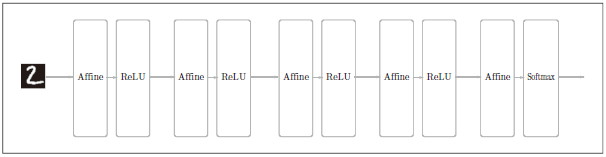
\includegraphics[width=0.9\linewidth]{chapter3_3.png}
    \caption{全连接网络结构示意图\cite{luyujie_216}}
    \label{fig:chapter3_3}
\end{figure}
\begin{figure}
    \centering
    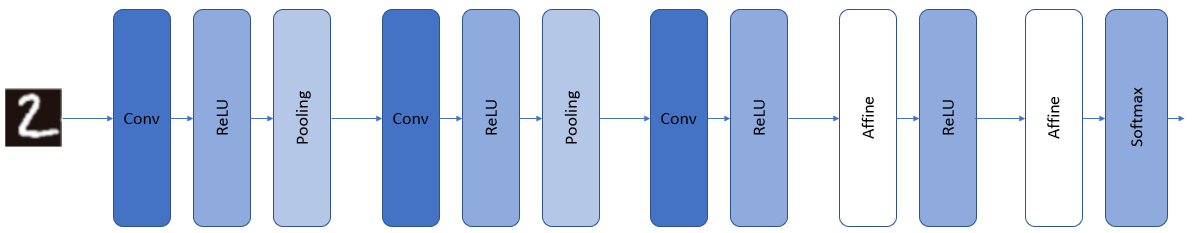
\includegraphics[width=0.9\linewidth]{chapter3_2.png}
    \caption{卷积神经网络结构示意图\cite{luyujie_216}}
    \label{fig:chapter3_2}
\end{figure}

如图\ref{fig:chapter3_2}所示,这就是一个卷积神经网络的例子,卷积神经网络中增加了卷积层和池化层。卷积神经网络的单个层连接的顺序是卷积层,激活函数层和池化层,其中池化层有时可以省略。
这样的组合方式可以被理解为前面的全连接层和激活函数层组合连接被替换成了卷积层,激活函数层和池化层的连接。另外,在如图\ref{fig:chapter3_2}所示的卷积神经网络中,靠近后面的输出层中使用了全连接层和激活函数层ReLU的组合。
然后,最终的输出层中则使用了全连接层和Softmax的组合。这样的搭配一般都是卷积神经网络中较为常见的搭配结构。

\subsection{卷积神经网络的原理}
在全连接的神经网络中,每一层都是通过全连接层组织起来的。在全连接的层次中,各个神经元都是连接在一起的,全连接的网络的输出数量是可以任意指定的,没有数量上的限制。

这样的结构会带来一定的问题,那就是数据的形状特征没有被充分地利用起来。用图片来举例,神经网络输入图片时,图片数据的格式一般是长、宽和高。长和宽代表图片以像素为单位的长度和宽度,高代表图片采样通道的宽度。
然而,这样的数据结构输入到全连接层搭建的神经网络中时,就会被展开成一维的数据。举例说明,MNIST的数据集中一张图片的长是28个像素点,宽是28个像素点,高度是1个通道(图片颜色为灰色色阶)。这样的形状输入到全连接的网络中前会被展开成一列,就是784个数据点输入到网络中。
图片一般是三维的形状,这样的形状结构中包含了重要的空间位置关系信息。比如通道与通道之间的关联信息,空间上相互距离比较接近的像素点一般具有相似的值,距离比较远的像素点一般没有关联。因此三维形状的数据中可能会蕴藏很多可以挖掘的特征模式。全是全连接层的神经网络就会把数据展开成一维数据,从而没有充分利用图片中的空间位置信息。

卷积神经网络就不会这样,图片输入到网络中就是以三维数据的格式输入,一个卷积层处理好数据以后,仍然会以三维的格式输入到下一个卷积层中。所以,卷积神经网络对于理解图像这样带有空间位置信息的数据是很有优势的。

\subsubsection{卷积层}
卷积运算发生在卷积层,卷积运算的计算过程类似滤波处理的过程。因此用于卷积运算的卷积核有时又被称为滤波器。常规的卷积运算如图\ref{fig:chapter3_4}所示。图中展示的便是一次二维卷积运算的过程。输入数据的尺寸是4乘4,卷积核的尺寸是3乘3,没有边界填充的情况下,最终输出结果的尺寸是2乘2。
\begin{figure}
    \centering
    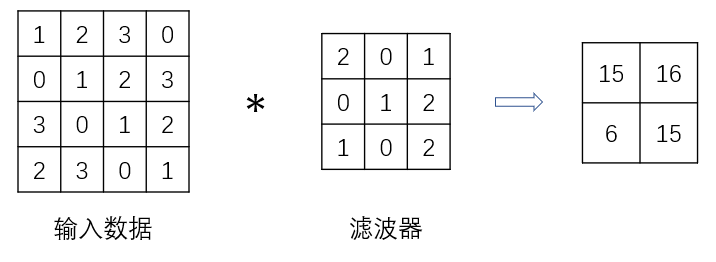
\includegraphics[width=0.9\linewidth]{chapter3_4.png}
    \caption{简单的卷积运算\cite{luyujie_216}}
    \label{fig:chapter3_4}
\end{figure}

卷积运算的具体过程是什么样的呢?下面结合图片\ref{fig:chapter3_5}来具体说明。如图\ref{fig:chapter3_5}中的第一行所示,第一行灰色区域代表第一步卷积操作所发生的区域,这个区域内的数字和卷积核的形状是相同的,所以区域内的数字可以与卷积核中对应位置的数字相乘,然后再把这些相乘的结果相加就得到了第一个结果。
运算后将结果保存到相应的位置。如图\ref{fig:chapter3_5}第二、三、四行所示将上面讲的过程在每个位置计算一遍,于是就完成了一次卷积运算。
\begin{figure}
    \centering
    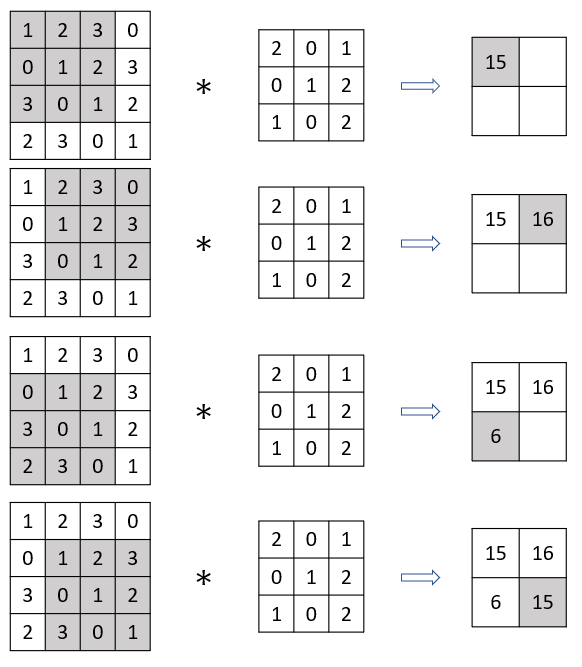
\includegraphics[width=0.9\linewidth]{chapter3_5.png}
    \caption{卷积运算过程示意图\cite{luyujie_216}}
    \label{fig:chapter3_5}
\end{figure}

和全连接的网络相同,卷积神经网络中除了网络的权重之外,还有偏置。卷积神经网络中偏置的个数一般就是卷积核的个数,而且每个卷积核对应的偏置的维度一般是1乘1。
计算完卷积之后,在相应结果的每个位置再加上偏置数字便得到了最终输出的数据,其计算过程如图\ref{fig:chapter3_6}所示。
对于输入数据,滤波器(维度是3乘3)与输入数据(维度是4乘4)进行卷积元算后便得到了初步的输出结果(维度是2乘2)。之后再将这个结果的每一个位置加上该卷积核对应的偏置数值,得到了最终结果(维度是2乘2)。
\begin{figure}
    \centering
    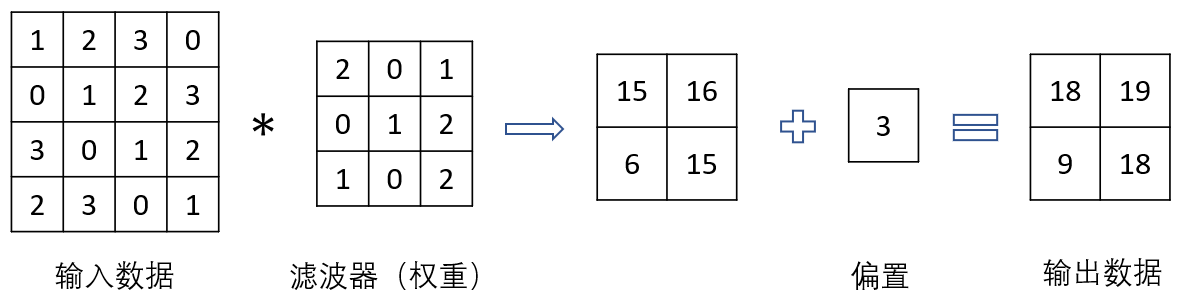
\includegraphics[width=0.9\linewidth]{chapter3_6.png}
    \caption{卷积运算后的偏置\cite{luyujie_216}}
    \label{fig:chapter3_6}
\end{figure}

三位卷积运算与二维卷积运算不同的是,卷积核的维度从2维提高到了3维,除了有长和宽的信息,还有通道数的维度。如图\ref{fig:chapter3_7}所示,以3通道为例,其运算过程与二维相似,先将对应位置的数字相乘,然后将相乘之后的结果相加,便得到了输出结果。
\begin{figure}
    \centering
    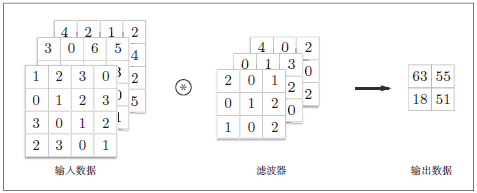
\includegraphics[width=0.9\linewidth]{chapter3_7.png}
    \caption{3通道的卷积运算\cite{luyujie_216}}
    \label{fig:chapter3_7}
\end{figure}
\subsubsection{池化层}
为了减少参数的数量,提高神经网络泛化能力,在卷积神经网络进行卷积运算以后,通常会进行池化操作。池化操作会同时减少卷积操作结果的长度和宽度。其运算过程如图\ref{fig:chapter3_8}所示。在第一行,图中灰色区域就是池化操作的一个操作单元,这个操作单元的大小来自池化操作的输入参数。
池化操作的输入是图中灰色区域内的数字,输出是一个数字。中间的运算过程一般有两个算法,一种是取所有数字中最大的数字,这种算法一般被称为最大池化操作;另外一种算法是取区域内所有数字的平均数,这种算法一般被称为平均池化操作。
\begin{figure}
    \centering
    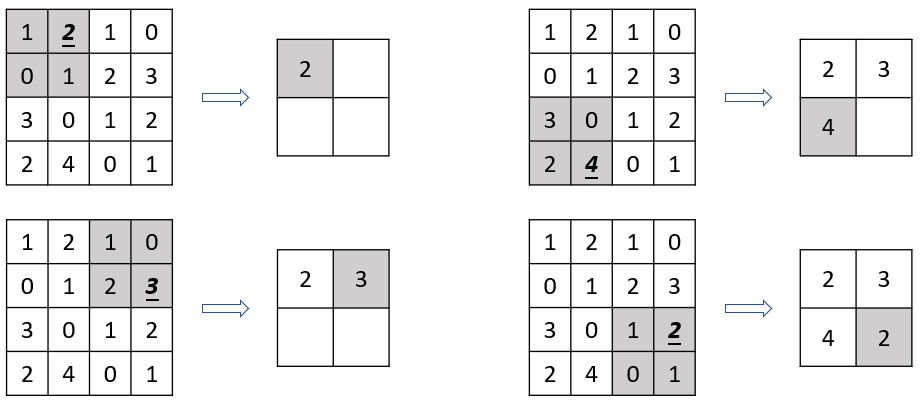
\includegraphics[width=0.9\linewidth]{chapter3_8.png}
    \caption{池化操作流程图\cite{luyujie_216}}
    \label{fig:chapter3_8}
\end{figure}

池化层与卷积层不一样的是,池化层没有训练参数,它的输入参数都是运算之前系统已经规定好的。池化层就是一个固定算法的函数。它另外一个特点是,池化操作后通道数是不变的,各通道是相互独立的,如图\ref{fig:chapter3_9}所示。
\begin{figure}
    \centering
    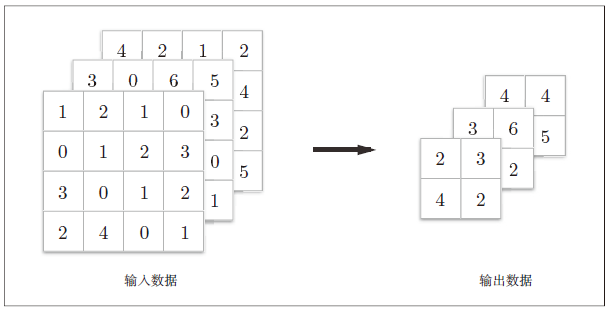
\includegraphics[width=0.9\linewidth]{chapter3_9.png}
    \caption{三维数据的池化操作\cite{luyujie_216}}
    \label{fig:chapter3_9}
\end{figure}

加入池化层后,神经网络对输入数据发生的一些微小干扰具有很好的鲁棒性。如图\ref{fig:chapter3_10}所示,即使图片发生了微小偏移,经过池化操作后,其特征仍能被准确地识别出来。
\begin{figure}
    \centering
    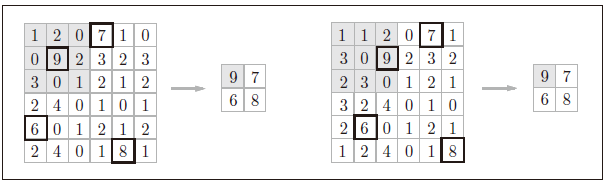
\includegraphics[width=0.9\linewidth]{chapter3_10.png}
    \caption{池化操作对发生偏移的输入具有鲁棒性\cite{luyujie_216}}
    \label{fig:chapter3_10}
\end{figure}

\section{卷积神经网络的分层抽象特性}
\subsection{人类视觉信息处理原理}
1981年来自美国的科学家David Hunter Hubel和来自瑞典的科学家Torsten Wiesel被授予了诺贝尔生理学或医学奖,以表彰他们在人类视觉系统信息加工领域做出的杰出贡献。
他们在人类视觉系统信息加工领域的工作贡献了当今神经生物学教科书视觉部分一半的内容,成为所有研究神经生物学方向学生的必学内容,这篇回忆录\cite{Hubel1998EarlyEO}中记录了他们一起做研究的过程。
在他们的这篇工作\cite{https://doi.org/10.1113/jphysiol.1959.sp006308}中记录了麻醉后的猫的大脑对不同光斑刺激的反应,并记录下了视觉皮层神经元的活动。
如图\ref{fig:chapter3_11}所示,他们在实验中发现,有一类细胞对一定范围视野内特定朝向上的刺激反应比较强烈,他们称这样的现象为朝向选择性,称这样的细胞为简单细胞。
这样的细胞仅对狭窄的视觉感受野有反应,刺激他们最好的方式就是用比较狭长的光斑,而且刺激的产生有明显的边界。当光斑覆盖整个作用区域时,并不能产生刺激反应。因此这样的细胞被看作是专门用来感受线条或边缘信号的接收器。
他们通过进一步的实验发现,还有一类细胞虽然对特定方向光斑的刺激有强烈反应,但是并没有明显的感受野。他们发现这样的细胞的上游是许多的简单细胞,接受简单细胞发过来的刺激信号。他们称这样的细胞为复杂细胞。
这种模式可以理解为复杂细胞是简单细胞的抽象,猫的视觉系统具有层级结构,图\ref{fig:chapter3_12}中展示了简单细胞和复杂细胞的关系。
\begin{figure}
    \centering
    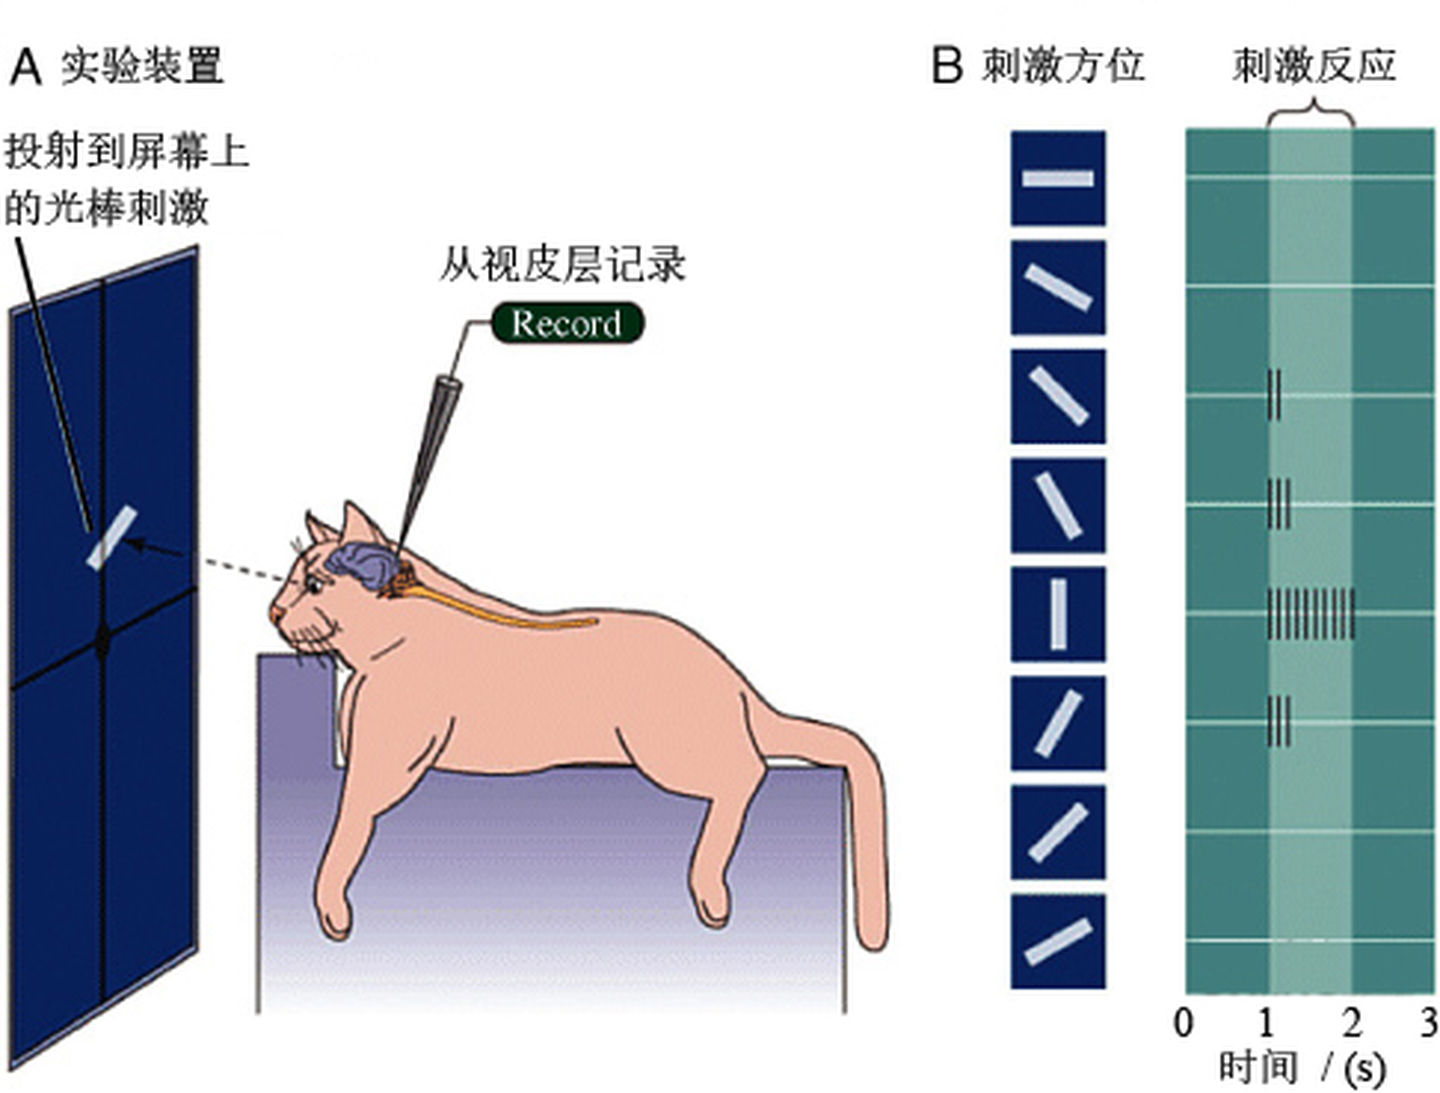
\includegraphics[width=0.9\linewidth]{chapter3_11.jpeg}
    \caption{使用光斑刺激猫的视神经,并记录猫的神经反应\cite{yanjianweishi}}
    \label{fig:chapter3_11}
\end{figure}

他们这样的发现对我们理解人类视觉信息加工的过程很有帮助。首先人类的视网膜接收外界传入的信号,经过简单细胞处理后,简单细胞完成了一些初级特征的提取,比如简单的直线或边缘信息。简单细胞后面有复杂细胞,复杂细胞负责完成更为抽象层次信号的处理,比如由各种方向的直线或边缘组成的形状信息。
我们由此可以推断,复杂细胞上面的细胞负责处理更为抽象的信息,经过一系列信息的抽象后,人类大脑就能识别看到的图像是一个什么物体,人类视觉信息加工是一个不断将信号进行抽象处理的过程。
\begin{figure}
    \centering
    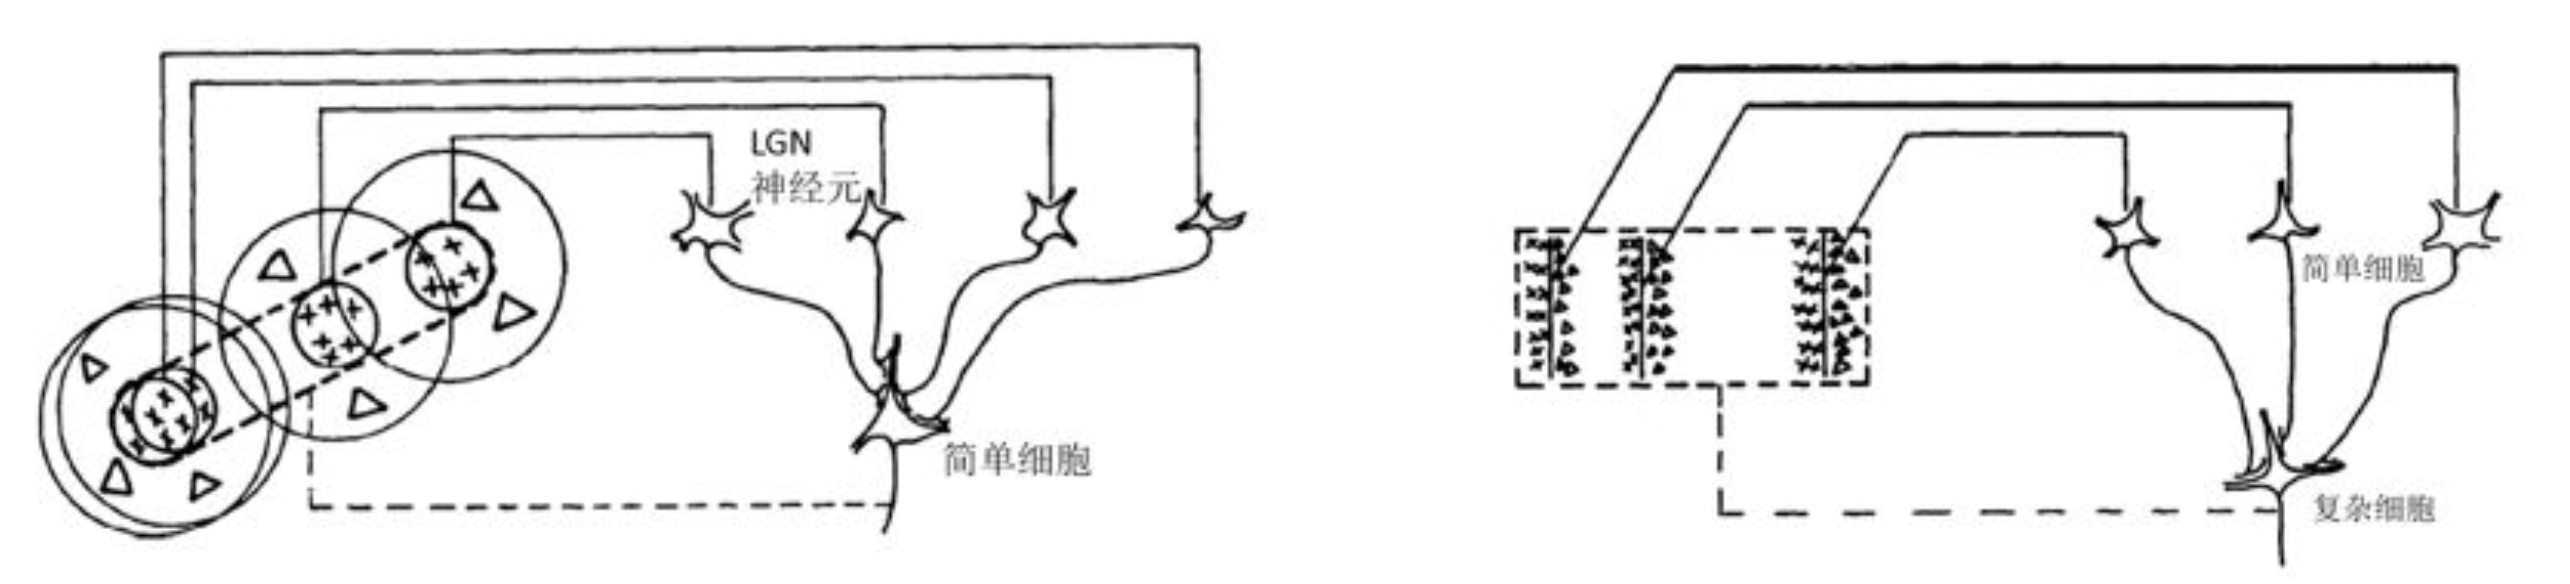
\includegraphics[width=0.9\linewidth]{chapter3_12.png}
    \caption{人类视觉信息处理过程中的简单细胞与复杂细胞\cite{yanjianweishi}}
    \label{fig:chapter3_12}
\end{figure}

\subsection{卷积神经网络的分层抽象特性}
在文献\cite{2019arXiv190906161K}中,作者提到了卷积神经网络是最接近还原人类视觉信息加工原理的人工神经网络。从卷积神经网络的基本原理中可以知道,卷积神经网络中的卷积核在与输入数据进行卷积操作时,具有类似人类视觉感受野中的朝向选择性。
随着输入数据在多层卷积层中逐层传递,一些特征信息逐渐被卷积核提取,提取的信息也逐步抽象。本文将卷积神经网络这种区别于其他人工神经网络的特性称为卷积神经网络的分层抽象特性。在卷积神经网络中,层数较低的卷积核提取的是较为初级的基本特征,层数较高的卷积核提取的特征是比较抽象的特征。
如图\ref{fig:chapter3_13}所示, 图中上半部分展示了一个训练完成的8层卷积神经网络结构,下半部分则是参数渲染后的效果。我们可以看到第一个卷积层学到的信息是一些基础的信息,例如边和角;第三层学到了由边和角构成的类似材质的图案;第五层则学到了由图案构成的物体的某个部分;最后,全连接层学到的是整个物体本身。
由此可以看出在卷积神经网络模型中,越靠后面的层次感兴趣的特征越抽象(这里我们称离输入端较近的层次为前面层次,离输出端较近的层次为后面层次),这种现象就解释了我们所说的分层抽象特性。
\begin{figure}
    \centering
    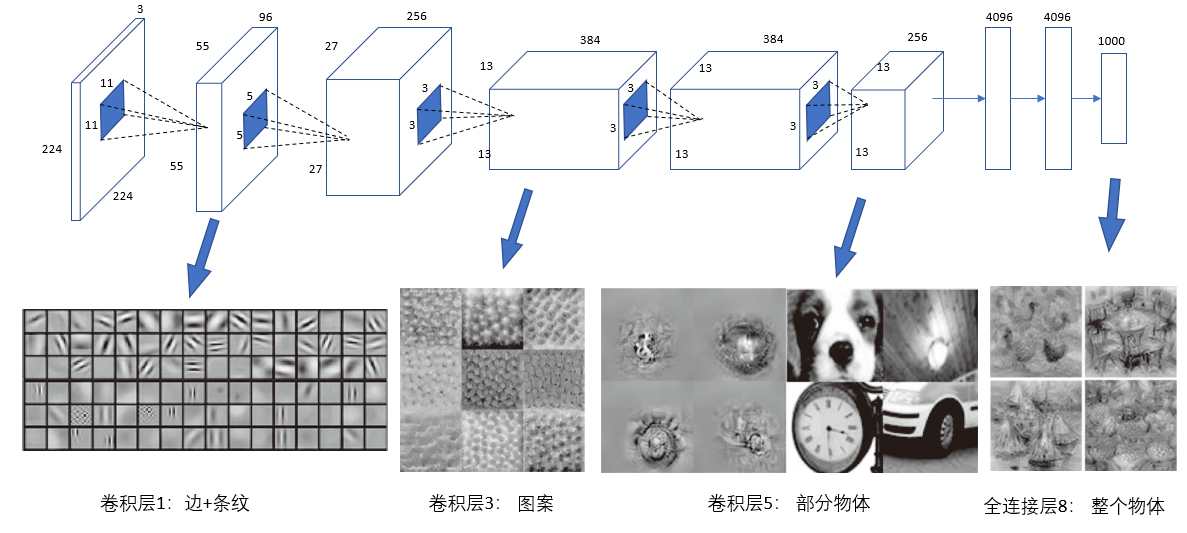
\includegraphics[width=0.9\linewidth]{chapter3_13.png}
    \caption{卷积神经网络的分层抽象特性示意图\cite{luyujie2018}}
    \label{fig:chapter3_13}
\end{figure}

\section{基于卷积神经网络的遗忘方法}
\subsection{遗忘方法的思路介绍}
我们首先来讨论什么是遗忘。对一个已经使用某数据训练的某神经网络而言,其理想的遗忘效果是,就好像一个神经网络模型从来没有使用遗忘数据训练过一样。换一个角度考虑,一个用户之所以会选择让模型遗忘自己的数据,其初衷是不希望自己的数据由于模型攻击而造成信息泄露。
当前的攻击方法有多种多样,我们无法也不可能去针对每种攻击方法去设置防御方法。我们能做的就是消除信息,换句话说,消除的信息越多,攻击者得到的信息就越少。消除信息的极限就是重新训练。
然而重新训练的代价是十分巨大的,一个神经网络模型少则几千个参数,多则高达数亿参数,重新训练的代价是十分昂贵的。所以完全消除所有信息看起来是不现实的。
那么有没有一种折中方案,既可以消除信息,又不用重新训练付出那么多代价?答案是肯定的,那就是我们不用消除所有的信息,只消除一部分抽象信息,一些基本的信息是分类无关的,攻击者即使拿到也没有用途。
这就用到了卷积神经网络特有的分层抽象特性,就像人类视觉信息处理过程一样,卷积神经网络较低层次的卷积层只提取了较为基本的视觉元素,比如边、角、简单的条纹等等。随着网络层次的提高,抽象程度逐渐提高,卷积核的感受野也逐步扩大,从而能提取到更为抽象的信息,比如一些有固定模式的组织,图案等。
到卷积神经网络比较高的层次后,感受野进一步扩大,从而能提取到跟分类息息相关的本质特征,比如不同人脸的区分,以及不同物体的区分,例如如猫和狗,飞机和卡车等。
一个攻击者最希望获得哪一部分的信息呢?毫无疑问是和分类有关的本质特征信息,而不是那些比较基本的边和角的信息。因为仅有边和角的信息是没用的,这些边和角的信息即使不用某个特定类别的数据训练也是可以得到的。
沿着这个思路,于是我们就想出了一个既可以消除信息,又能不用全部参数参与训练的折中方案,那就是消除层数靠后面的抽象信息,其方式是重置靠后面层次的网络参数。
重置靠后面层次的网络参数之后会带来一个问题,我们不仅消除了要遗忘数据的较高层次的抽象信息,同时也消除了保留数据的较为重要的抽象信息。为了解决这个问题,我们想到了用保留集去重新训练网络的方法。
这里说的重新训练不是指要训练所有的网络参数,而是只训练我们前一步骤重置的层次较高的网络参数。其目的是恢复那些保留类别的高层次的信息。这一步骤我们的做法是使用保留类别的训练数据去训练这一部分参数。等待模型收敛之后,我们就可以得到想要的网络。具体过程如图\ref{fig:chapter3_14}所示。
\begin{figure}
    \centering
    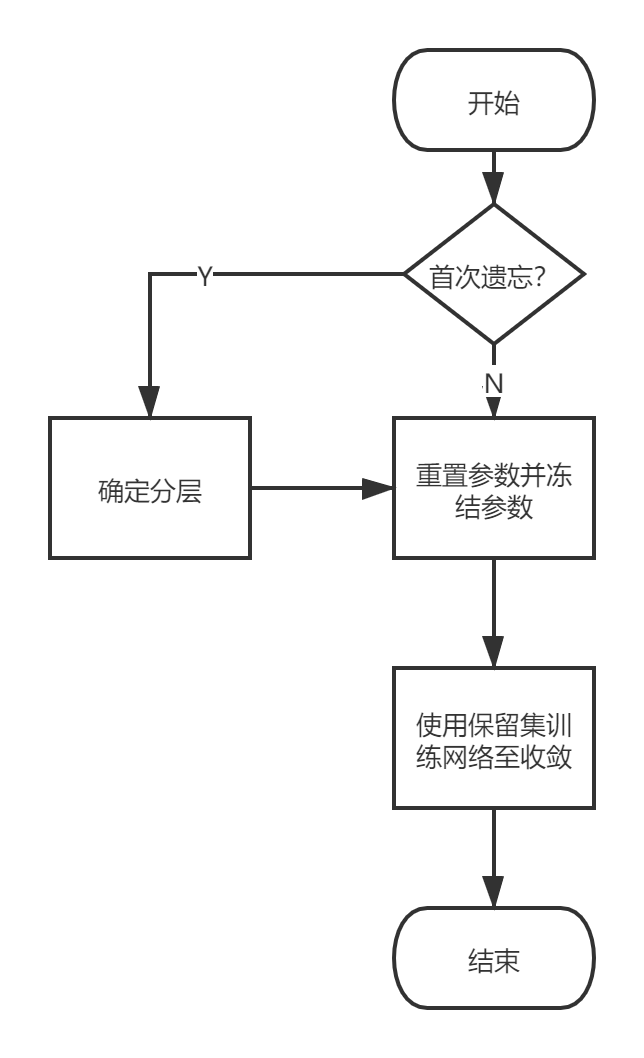
\includegraphics[scale=0.35]{chapter3_14.png}
    \caption{遗忘方法流程图}
    \label{fig:chapter3_14}
\end{figure}

\subsection{确定分层}

前面小节讨论了遗忘方法的思路方案。随之而来的问题就是,我们需要重置一定层数的网络参数,我们究竟要重置多少层呢?重置层数的多少直接影响了遗忘效果的好坏以及重新训练的时间,因此确定分层数量是本方法的一个重要环节。

为了确定重置参数的层数,我们要综合考虑评价遗忘效果的各个指标。首先我们要考虑在哪一层重置参数才可以在遗忘集上达到较低的准确率,并且不影响保留类别的准确率。
选择这个指标的因素是出于实际应用的考虑,因为我们训练神经网络模型的目的是分类,所以一个基本的要求就是要有较高的分类准确率。然后站在用户的角度考虑,我们需要将用户要遗忘的类别很好的遗忘掉,所以我们又不希望遗忘的类别具有较高的准确率。
另外一个需要考虑的因素是重新训练的时间,这也是本文十分看重的一个指标。机器学习的遗忘一个很朴素的方法就是重新训练,可是重新训练会很耗费时间。本文想到了利用了卷积神经网络的分层抽象特性,使得不用完全重新训练即可达到与重新训练相近的准确率。
因此,重新训练时间也是一个很重要的考虑因素,即选择的重置参数的层次并且训练后,网络训练过程从开始到最终收敛的时间不能太长。
还有一个很重要的指标就是训练后与完全重新训练网络的激活距离,这个距离越近越好,其目的是为了防止成员推断攻击。因为有时候一些类别遗忘以后,攻击者可以根据网络的输出结果判断出一些输入数据有没有被用于网络训练。我们不希望一些类别遗忘以后能够被推断出曾经参与过训练。

有了上述确定分层的指导原则,我们就可以对分层方法进行评价。还有一个问题没有被解决,就是我们需要在每次执行遗忘算法的时候都确定分层一次吗?
在本方法中我们无需在每次遗忘时均评价一次分层效果。对同一个网络结构,同一套网络训练数据集,我们仅需在首次遗忘时进行分层效果的测试,在后续的遗忘训练时,只需要使用首次遗忘时使用的分层数。遗忘可持续性实验的实验结果将会证明这一点。

\subsection{重置并冻结参数}

重置并冻结参数的原因是为了减少遗忘数据在原网络中的信息,并且保留和分类关系不密切的基本信息。对于重置和冻结参数,我们将分开进行解释。
我们来看参数应当如何初始化,如果初始化参数不当,会给我们带来很大的麻烦。比如模型无法收敛,或者会产生无法达到全局最优等问题。
为了防止这样的由于参数初始化不当而带来的问题,我们选取的策略是,保存模型初始化参数。当网络中某些层次需要重置参数时,我们将保存下来的相应层次的网络参数补充到需要重置参数的层次当中。
这样做的一个出发点是,既然这个网络模型初始化参数能够使得网络达到收敛状态,就说明这个参数是一个较为合理的初始化参数,没有均值过大或过小,或方差过大或过小的异常情况。经过实验证明,这种做法能够达到理想的效果,在实验中并未发现由于重置参数不当而带来的网络训练无法收敛的问题。

对于冻结网络,我们需要关注的问题是冻结网络的必要性方面,即到底需不需要冻结网络。为了探究是否需要冻结参数的问题,本文也设计了专门冻结参数与非冻结参数训练的对比实验,实验过程和结果将在本文第四章集中展示。

\subsection{训练网络}

在重新训练网络时,使用的数据集是原来的数据集减去要遗忘类别的数据集。因为是原数据集和遗忘数据集的差集,为了便于表达,以下称之为保留集。重新训练网络的目的是为了还原保留类别的信息。因为重置了一部分网络参数后,所有的训练数据中涉及到的分类信息已经全被消除掉了。
此时网络攻击者根据网络输出还原训练数据的信息几乎是不可能的。为了保证保留类别还原重置参数以前的效果,我们使用保留集对重置的参数进行还原。

在重新训练网络的过程中,待更新的参数数量对比完全重新训练的参数数量,少了冻结层次的参数,因此训练网络中不需要对冻结的参数计算梯度。
因此从理论上看,网络参数的收敛速度应当有一些减少。为了检验训练速度能够提升多少,我们专门设计了对比实验,分别记录了完全重新训练所花费的时间和使用本文遗忘方法训练所需要花费的时间。

再有,对于遗忘方法,不能忽视的是遗忘的可持续性问题。随着遗忘方法使用次数的增多,使用本文方法遗忘后的网络性能和完全重新训练网络的性能之间的差距是否会越来越大呢?为了验证这一问题,我们专门设计了连续遗忘对照实验。

\section{遗忘效果的衡量指标} \label{forget_evaluation_index}

了解了一些关于卷积神经网络遗忘的概念之后,我们也要了解遗忘到什么程度才能算是比较好的遗忘效果。为此,我们设计了一些用来评价遗忘效果的指标。这些指标可以帮助我们从各个方面了解当前网络模型的训练状态。这些指标有测试准确率、收敛时间和激活距离。
\subsection{测试准确率}

训练神经网络的过程中,我们不仅要利用训练数据去训练网络,也需要用测试集去测试训练网络的泛化成果,目的是为了检测训练的网络是否出现过拟合情况。我们将测试集根据遗忘需求分为两个部分,仅有遗忘类别的测试遗忘集和仅有保留类别的测试保留集。
使用测试遗忘集的测试结果可以反映网络对于遗忘类别的遗忘程度。单从测试准确率这一个指标上来看,在测试遗忘集上的准确率越低,代表对遗忘类别遗忘效果越好。
同理,使用测试保留集的测试结果可以反映网络对于保留类别的保留情况。单从测试准确率这个指标上来看,在测试保留集上的准确率越高,代表保留类别的保留效果越明显。

但是并不是保留效果越高,遗忘效果越低,遗忘的效果就越好。这两个指标只是对网络学习结果的一个参照。为了综合评价遗忘效果我们还要参照激活距离(公式\ref{index_distance})和收敛时间。

\subsection{收敛时间}

收敛时间用于衡量本文遗忘方法在时间上的节约程度。规定从用保留集进行训练开始,到当前训练批次损失函数输出的平均值小于一定限值为止,这中间过程的训练批次数称为收敛时间。

这么定义的目的是因为具体的时间间隔会因实验环境的不同而不同,比如实验用的CPU,内存,硬盘,显卡,神经网络结构和数据集等都有可能发生变化,因此我们要寻找一个既能反映训练过程长短又能不随实验环境变化的量。
训练批次数刚好符合这个条件,因为只要每批训练的参数(即BATCH\_SIZE)是固定的,每个BATCH的训练批次数(即Epoch数)就是一定的。无论训练环境如何变化,虽然训练用的整体时间会有变化,但是Epoch数是不变的。

为了便于实验,我们给收敛时间确定一个计算公式。我们将收敛时间定义为网络训练过程中,本轮Epoch中平均的损失函数值首次下降到指定阈值时所花费的Epoch数。在本文的实验中取了三个阈值,分别是0.1,0.05和0.03。

之所以会将从保留集开始训练的时刻作为起始时间,是因为下面的确定分层步骤是一次性的步骤,对于同一个网络结构,同一个数据集,确定网络分层仅在进行第一次遗忘操作时需要操作一次。
重置和冻结参数操作是固定程序的操作,通过脚本即可完成。所以相比训练过程的时间,这个操作的时间我们暂且不记。

\subsection{激活距离}

激活距离是指遗忘后模型与完全重新训练模型在测试集上的平均距离。它用于衡量遗忘后模型与完全重新训练模型在网络输出结果上的相似程度。它的计算公式是
\begin{equation}
I_{distance} = {\mathbb{E}}_{x\in {\mathcal{D}_{test}}}[{\Vert softmax(f_w(x)) - softmax(f_{w_{\mathcal{D}_R}}) \Vert}_2 ] \label{index_distance}
\end{equation}

$f_w(x)$代表完全重新训练网络的输出结果,$f_{w_{\mathcal{D}_R}}$代表使用本文遗忘方法训练网络的输出结果。
它们输出结果softmax函数的差值向量的第二范数在测试集上的期望,就是激活距离。


\section{本章小结}
本章对本文所使用的遗忘方法做了系统性的描述。为了讲清卷积神经网络的分层抽象特性,本章首先介绍了卷积神经网络技术的基本原理,包括卷积操作以及卷积层和池化层的作用。
其次依托于人类视觉信息处理的原理,介绍了卷积神经网络的分层抽象特性,这也是本文所使用方法的理论依据。
再次介绍了本文所使用的遗忘方法,可以分为三步,即确定冻结层次,重置和冻结参数还有训练网络。最后介绍了本文用来评价遗忘效果的主要指标,包括测试准确率、收敛时间和激活距离。
